\section{Desplazador lógico \label{sec:s1}}

\begin{center}
	\begin{minipage}{12cm}
		\begin{tcolorbox}[title=Actividad 1]
			Completar el código del desplazador lógico utilizando concatenaciones en el lenguaje de su elección. Compilar y simular. Configurar en la tarjeta DE2-115 asignando \textit{switches} y \textit{LED's}. Datos de 8 bits.
		\end{tcolorbox}	
	\end{minipage}
\end{center}

La visualización RTL del desplazador lógico en Verilog se muestra en la \autoref{fig:logical_shifter_rtl}. En el visor se tiene un decodificador conectado junto con 8 multiplexores (uno por cada bit a la salida). Las simulaciones para el código en Verilog se visualizan en la \autoref{fig:logical_shifter_WaveBi}. Los bits a la entrada fueron escogidos de tal forma que se observe de manera clara el corrimiento a la izquierda.

En los Anexos se localiza la descripción del desplazador lógico. Se observa que la descripción se hizo utilizando una lista sensible para los puertos de entrada y selección. Dentro de esta estructura se empleó la sentencia \textit{case} para indicar como se debe comportar la salida con respecto a la variable de control SEL. Cabe resaltar que para el desplazamiento lógico a la izquierda se concatenaron los bits menos significativos de la entrada a la izquierda y valores en bajo a la derecha. En caso de que se hubiera hecho un desplazamiento a la derecha, se debe hacer la concatenación de valores en bajo a la izquierda y los bits más significativos de la entrada a la derecha.

\begin{figure}[ht]
	\centering
	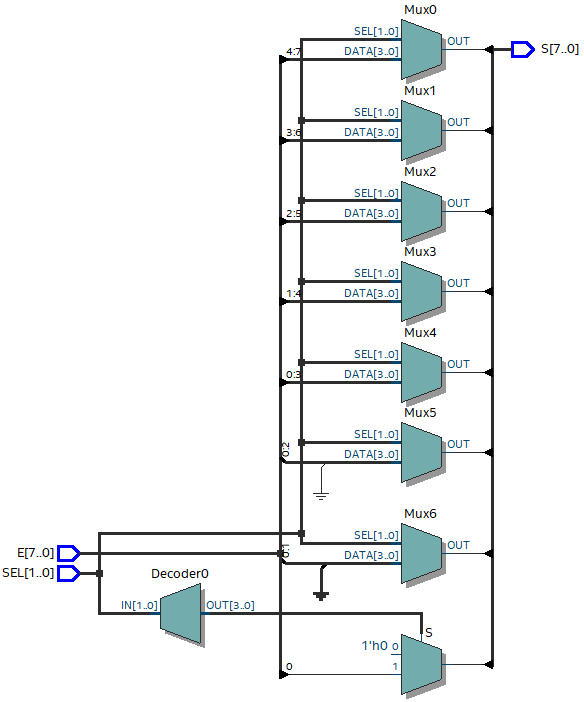
\includegraphics[scale=0.8]{Logical_Shifter_RTL.png}
	\caption{Diagrama RTL del desplazador lógico de 8 bits. \label{fig:logical_shifter_rtl}}
\end{figure}

\begin{figure}[ht]
	\centering
	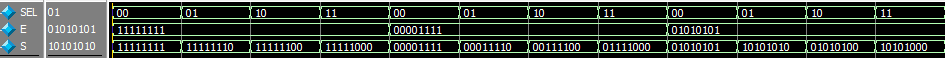
\includegraphics[scale=0.65]{Logical_Shifter_WaveBi.png}
	\caption{Simulación del desplazador lógico con el visor de formas de onda de ModelSim. \label{fig:logical_shifter_WaveBi}}
\end{figure}